\documentclass{article}
% --- watermark (auto-inserted) ---
\usepackage{xcolor}
\usepackage{xfp}% \fpeval; in the kernel since 2022, harmless on older LaTeX
\usepackage{draftwatermark}
\newlength{\watermarkTextWidth}
\AddToHook{begindocument/end}{%
  \SetWatermarkText{\normalfont Generated by The Agentic Scientist}%
  \SetWatermarkFontSize{10pt}%
  \SetWatermarkLightness{0.85}%
  \settowidth{\watermarkTextWidth}{\normalfont\fontsize{10pt}{12pt}\selectfont Generated by The Agentic Scientist}%
  \edef\watermarkScale{\fpeval{0.8 * sqrt(\paperwidth**2 + \paperheight**2) / \watermarkTextWidth}}%
  \edef\watermarkAngle{\fpeval{atand(\paperheight/\paperwidth)}}%
  \SetWatermarkScale{\watermarkScale}%
  \SetWatermarkAngle{\watermarkAngle}%
}
% --- end watermark ---

\usepackage{paper,times}
\usepackage{amsmath,amssymb,booktabs,graphicx,subcaption}
\usepackage{hyperref,xurl}
\newcommand{\sigmoid}{\operatorname{sigmoid}}
\newcommand{\Exact}{\textsc{Exact-refit}}
\title{Exact-Refit Audits of Pairwise Ranking Sensitivity}

\begin{document}
\maketitle

\begin{abstract}
Pairwise-comparison leaderboards compress observed outcomes into an ordered list, but the stability of that list depends on which observations remain. We study a constrained deletion audit for regularized Bradley--Terry rankings: clean-fit influence values define nested deletion prefixes, a bounded shortlist of contenders is compared by retained-data refits, and an independent solver measures the resulting ranking changes. Evaluations cover crowdsourced Chatbot Arena preferences and historical basketball outcomes at three small deletion fractions. Averaged over settings and budgets, the studied selector inverts 1.172\% of participant pairs, compared with 0.934\% for high-loss deletion and 0.390\% for random deletion. This aggregate hides important exceptions: high-loss deletion is more disruptive on Arena at the larger budgets. Fixed-mask group-weight resampling also gives opposite high-loss-relative orderings across the datasets. These are conditional perturbation results, not uncertainty for a reoptimized deletion procedure or evidence of a causal effect of evaluation design. The contribution is an auditable, setting-specific sensitivity assessment rather than a universal ranking attack or a guarantee of stability.
% @evidence[[paper_data.json#/final_evaluation/metrics]]
% @evidence[[paper_data.json#/final_evaluation/evaluation_evidence/episodes]]
\end{abstract}

\section{Introduction}
Pairwise judgments are a natural interface for evaluation: a voter chooses between responses, or a game produces a winner and a loser. A ranking model turns these local outcomes into global scores. Such scores are useful precisely because they reduce a complex comparison graph to a compact summary. That compression also makes it difficult to tell which observations sustain a displayed ordering. Sampling uncertainty, dependence between observations, and targeted changes to the observed sample need not affect that ordering in the same way.

We ask a deliberately finite-sample question: \emph{how much does a fitted ranking change when a small, explicitly constrained subset of its observed comparisons is removed?} This is not an assessment of the true quality of a model or team. The reference is the ranking fitted before deletion, not an external ground-truth ordering. A large change indicates sensitivity of that fitted summary; a small change under a particular rule does not certify robustness to every equally sized subset.

Our audit couples a local influence calculation with bounded exact-refit selection. For each possible challenger to the clean leader, influence values define an immutable ordering of rows. Deletions must be nested prefixes of that ordering. A screening calculation reduces the contenders considered by retained-data fits, while an independent evaluator checks the clean-fit certificate and refits each deleted dataset. This separation matters: an internally predicted rank reversal is not itself a measured ranking change.

The empirical scope is crowdsourced Chatbot Arena preferences and historical basketball outcomes, fitted with the same static Bradley--Terry objective. These settings provide contrasting sources of pairwise data without constituting a controlled intervention on evaluation design. We find greater aggregate disruption than the measured baselines, but the ordering of deletion rules depends on dataset and budget. Conditional resampling makes that dependence especially clear: the high-loss comparator is consistently more disruptive in the stored Arena resamples and less disruptive in the NBA resamples.
% @evidence[[paper_data.json#/final_evaluation/evaluation_evidence/episodes]]

The contributions are therefore narrow and verifiable: a source-inspectable frozen-prefix audit with independent refitting; a budget-resolved comparison against high-loss and random deletion on contrasting real-data settings; and an uncertainty analysis that explicitly separates repeated random masks from fixed-mask data reweighting. We do not identify a globally most damaging deletion set, isolate the causal contribution of shortlist refitting, or attribute the cross-setting differences to crowdsourcing rather than other dataset properties.

\begin{figure}[t]
  \centering
  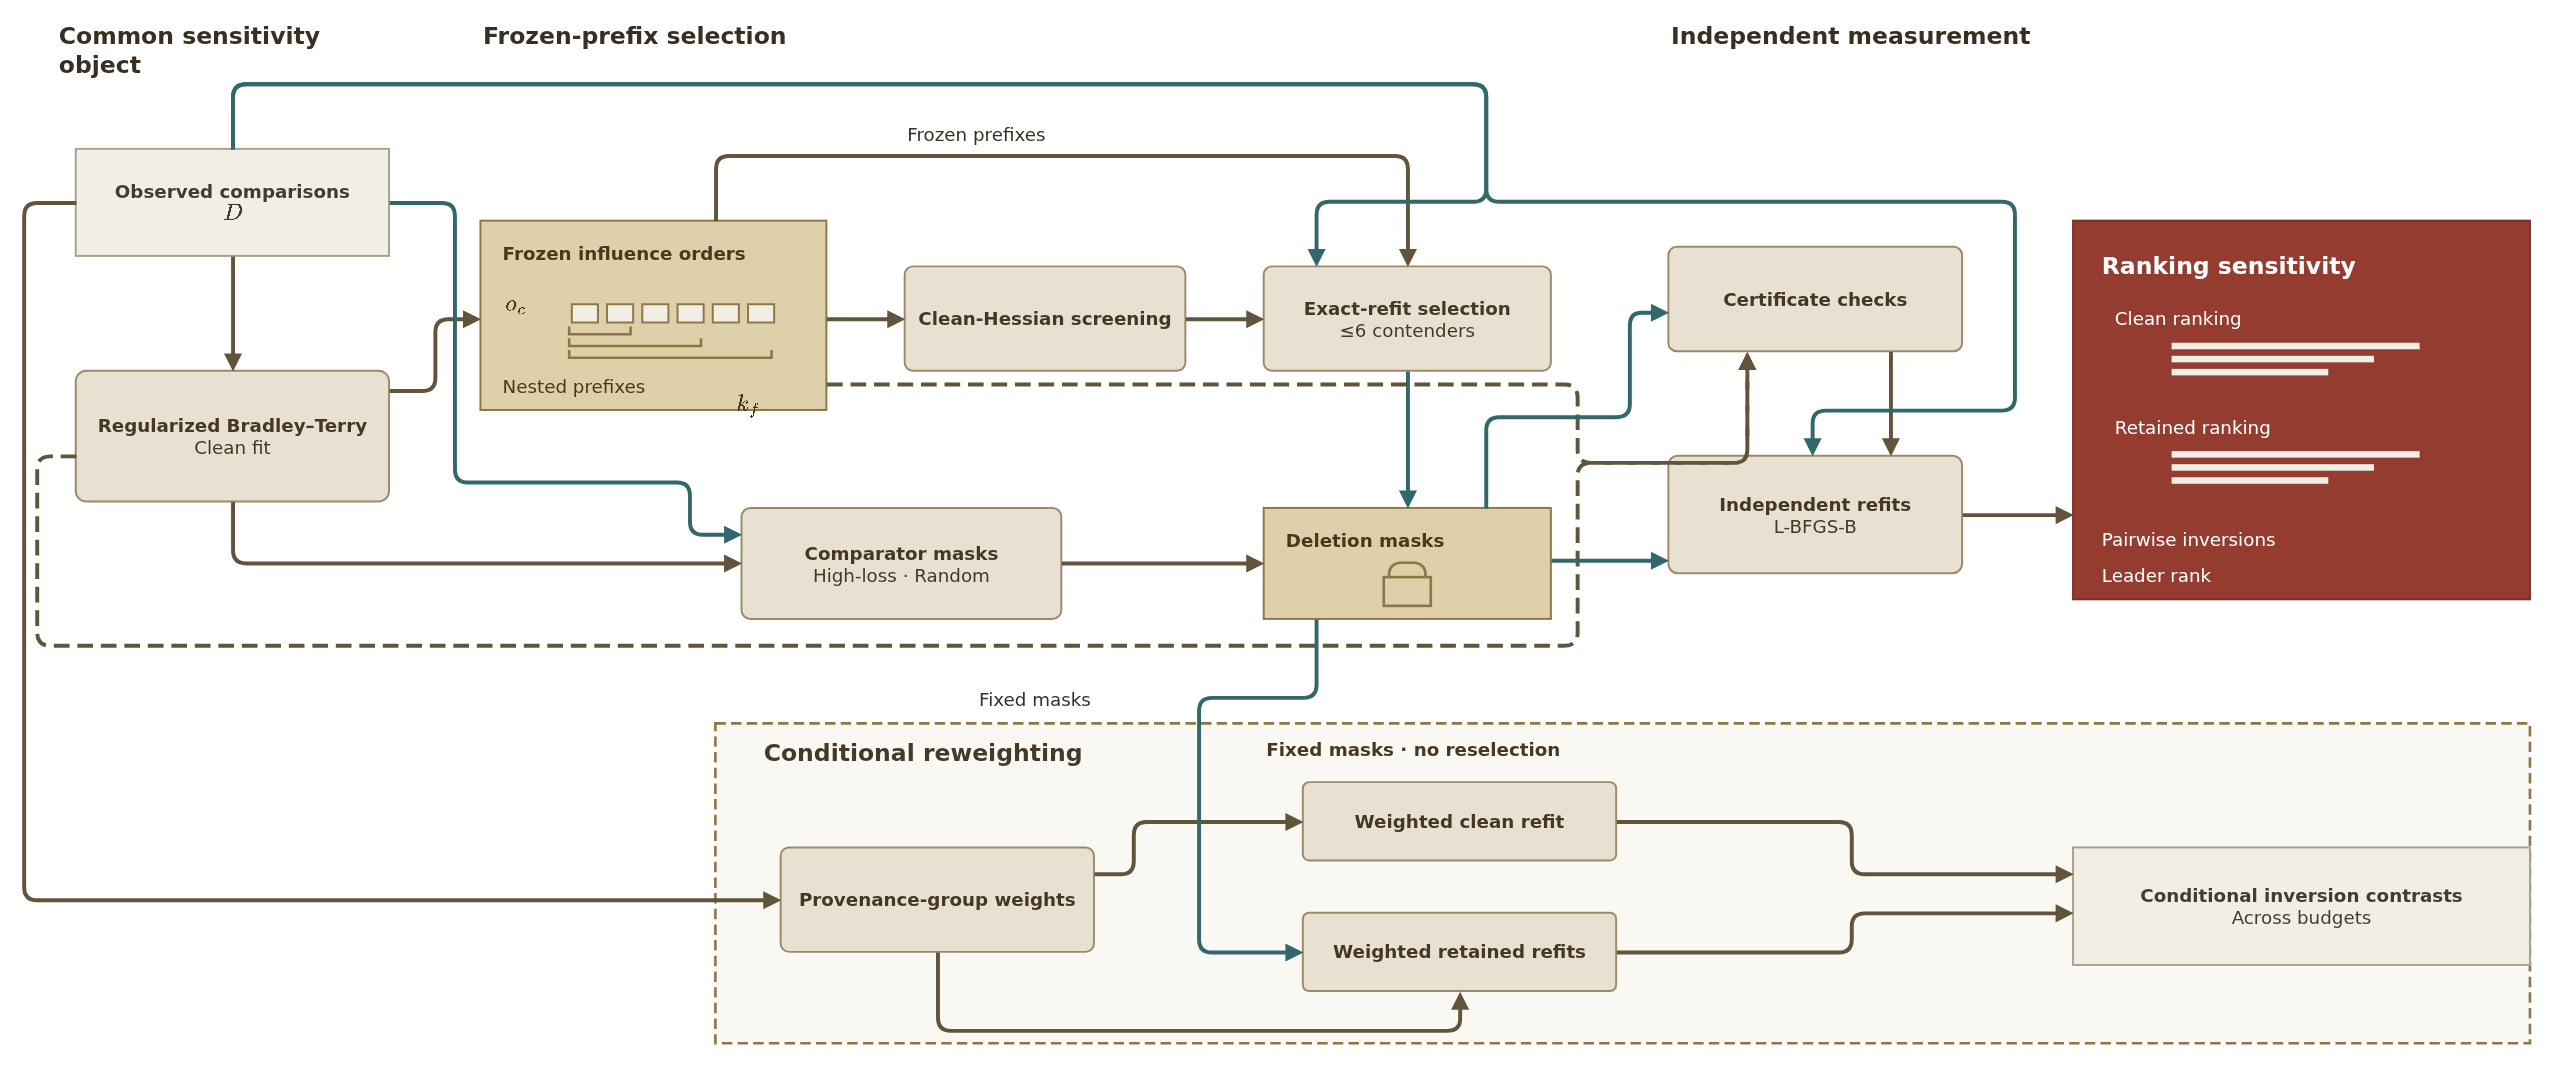
\includegraphics[width=0.98\textwidth]{figures/audit_overview.png}
  \caption{A common audit for contrasting pairwise-data settings. A regularized fit supplies clean influence orders; bounded contender selection uses retained-data refits without changing those orders. Independent refits measure disruption. The uncertainty branch reweights provenance groups with deletion masks fixed: it does not repeat contender selection.}
  \label{fig:overview}
  % @evidence[[source_evidence/selector.py#L145]]
  % @evidence[[source_evidence/evaluate_final.py#L831]]
\end{figure}

\section{Related Work}
\paragraph{Pairwise ranking.}
Probabilistic ranking has classical roots in tournament likelihoods and comparative judgment \citep{Zermelo1929,Thurstone1927}. Bradley--Terry modeling \citep{Bradley1952} and the binary-comparison ranking problem \citep{Ford1957} provide the immediate foundation. Generalized Bradley--Terry estimation and software support richer fitting procedures \citep{Hunter2004,Turner2012}; explicit tie models \citep{Davidson1970} and bias-reduced likelihood \citep{Firth1993} are distinct from the half-win ties and quadratic penalty used here. Models over permutations \citep{Plackett1975} address a related but different observation space. Rank Centrality and counting-based ranking study estimation and recovery from pairwise comparisons \citep{Negahban2012,Shah2017}. Our endpoint instead measures changes relative to an already fitted ordering, using a normalized inversion count related to rank-correlation statistics \citep{Kendall1938}.

\paragraph{Influence and sample removal.}
Influence curves formalize local sensitivity \citep{Hampel1974}, while observation diagnostics connect data perturbations to fitted parameters \citep{Cook1977}. Influence functions have also been used to trace predictions to training observations \citep{Koh2017}. The infinitesimal jackknife approximates weighted refitting \citep{Giordano2019}, and finite-sample removal robustness explicitly asks whether dropping a small subset changes a conclusion \citep{Broderick2020}. We use influence only to define and screen constrained deletion prefixes. Retained-data fitting evaluates those prefixes; it does not make the prefix family exhaustive or establish approximation-error bounds for our selection criterion.

\paragraph{Evaluation and conditional uncertainty.}
Chatbot Arena motivates the preference-ranking setting \citep{Chiang2024}. Vote-rigging research studies deliberate manipulation of that platform \citep{Min2025}; here the intervention is deletion from a fixed observed sample, not the collection of new strategic votes. Basketball records provide a second source of outcomes \citep{NBAdata}, not another language-model benchmark. Bootstrap methods distinguish the statistic being resampled from its reported uncertainty \citep{Efron1979,Davison1997}; the Bayesian bootstrap is a different weighting construction \citep{Rubin1981}. Clustered and crossed-data resampling require attention to dependence assumptions \citep{Field2007,Owen2007}. Our multinomial provenance-group weights are a conditional diagnostic, not a validated population uncertainty model for all dependencies in either dataset.

\section{Method}
\subsection{Problem setup and evaluation target}
Let $D=\{(a_i,b_i,y_i,u_i)\}_{i=1}^{n}$ contain observed comparisons of $m$ participants. Here $y_i\in\{0,\tfrac12,1\}$ is the outcome for endpoint $a_i$, and $u_i$ is a stable row key used only for deterministic tie resolution. Define $x_i=e_{a_i}-e_{b_i}$, margin $z_i=x_i^\top\theta$, and loss $\ell_i(\theta)=\log(1+\exp z_i)-y_i z_i$. The clean fit is
\begin{equation}
 \widehat\theta=\arg\min_{\mathbf{1}^\top\theta=0}
 \left\{L_D(\theta)=\frac{1}{n}\sum_{i\in D}\ell_i(\theta)
             +\frac{\lambda}{2}\|\theta\|_2^2\right\},\qquad \lambda=0.001.
 \label{eq:objective}
\end{equation}
% @evidence[[source_evidence/evaluate_final.py#L29]]
% @evidence[[source_evidence/evaluate_final.py#L653]]
Half-win outcomes use the same logistic cross-entropy, rather than an additional tie-probability parameter. A retained subset is fitted using its \emph{own} mean loss and the same $\lambda$. Consequently, deletion changes the likelihood contribution relative to the penalty; it is not equivalent to keeping a fixed sum-loss penalty.

Let $\pi(\theta)$ rank scores in descending order, with rounded-score ties broken by participant identity. For clean leader $l$, the primary endpoint is normalized pairwise inversion:
\begin{equation}
 I(D,R)=\frac{1}{\binom m2}\sum_{a<b}
 \mathbf{1}\!\left\{a,b\text{ have opposite orders in }
       \pi(\widehat\theta_D),\pi(\widehat\theta_{D\setminus R})\right\}.
 \label{eq:inversions}
\end{equation}
The secondary endpoint is the clean leader's new zero-based rank divided by $m-1$. Both describe fitted-ranking disruption; neither evaluates predictive accuracy. Budgets are $k_f=\lfloor fn\rfloor$ for $f\in\{0.001,0.005,0.01\}$. Equal row fractions provide a common sample-mass scale, but do not equalize participant exposure, graph topology, information loss, or difficulty across datasets.
% @evidence[[source_evidence/evaluate_final.py#L680]]
% @evidence[[paper_data.json#/final_evaluation/evaluation_evidence/episodes/0/solution/cases]]

\subsection{Rationale: local orders, retained-data decisions}
The design rationale is to use local sensitivity for a tractable family of deletions while measuring finite deletions by refitting. For every clean nonleader $c$, form $v_c=e_l-e_c$ and solve $Hd_c=v_c$, where $H=\nabla^2 L_D(\widehat\theta)$. The row influence for this contrast is
\begin{equation}
 q_{ic}=(\sigmoid(x_i^\top\widehat\theta)-y_i)x_i^\top d_c.
 \label{eq:influence}
\end{equation}
Ascending $q_{ic}$ gives an order $o_c$. The legal deletion at each budget is exactly $R_{cf}=o_c[1:k_f]$. The order is computed once from the clean fit and never rearranged after refitting. This restriction makes the output independently checkable, but excludes adaptive reorderings and arbitrary subset swaps.
% @evidence[[source_evidence/selector.py#L145]]

The screening calculation predicts full-vector displacement using the clean Hessian. Writing $g_i=\nabla\ell_i(\widehat\theta)$, it uses
\begin{equation}
 \widetilde\delta_{cf}=\frac{H^{-1}}{n-k_f}
       \left(\sum_{i\in R_{cf}}g_i+k_f\lambda\widehat\theta\right).
 \label{eq:screen}
\end{equation}
% @evidence[[source_evidence/selector.py#L181]]
The penalty correction follows from the retained-mean objective, not an extra intervention. The retained gradient at the clean optimum is $-(\sum_{R}g_i+k\lambda\widehat\theta)/(n-k)$; replacing retained curvature by $H$ gives Eq.~\ref{eq:screen}. The approximation can misorder contenders for finite deletions. Refitting the shortlisted prefixes addresses that particular approximation in the decision, but does not remove the shortlist restriction.

\subsection{Compared approaches and selection rule}
\Exact{} screens every nonleader by a lexicographic tuple: the sum of predicted leader-rank drops across budgets; the number of target-gap reversals; summed clipped relative gap closure; and preference for a better clean rank. A shortlist contains at most six contenders, retaining the screening maximizer and the clean runner-up. Each shortlisted contender's frozen prefixes are refitted under Eq.~\ref{eq:objective}, and the same tuple is evaluated using fitted, rather than predicted, scores. A reversal requires a leader--contender gap below $-10^{-8}$; relative closure is clipped to $[0,2]$. Incomplete refit sets are excluded. If none completes, selection falls back to the screening maximizer.
% @evidence[[source_evidence/selector.py#L138]]
% @evidence[[source_evidence/selector.py#L231]]

This selection rule targets leader demotion before other criteria, whereas the primary endpoint counts inversions anywhere in the list. Thus the method does not directly maximize Eq.~\ref{eq:inversions}. High-loss deletion instead sorts descending clean per-row logistic loss, using stable keys for ties. Random deletion uses one seeded permutation and its nested prefixes. These comparators use the same row budgets and independent retained-data solver. A no-deletion check refits the unchanged data; it is a numerical control, not a competing attack.
% @evidence[[source_evidence/evaluate_final.py#L949]]

We also retain descriptive development scores for clean-Hessian-only selection and a retained-curvature shortlist expansion in Supplementary Information. They are not controlled final-partition ablations. The final evidence evaluates the selected six-contender configuration against deletion baselines, not an isolated causal effect of exact-refit selection or extra curvature information.

\subsection{Implementation and independent verification}
The selector aggregates comparison counts and fractional wins by ordered endpoint pair. It uses centered Newton updates, Cholesky linear solves, a backtracking line search, warm starts across nested retained datasets, and a cache keyed by the removed row set. The independent evaluator instead starts L-BFGS-B fits from zero. It checks clean-score stationarity, the Hessian contrast solve, row influence values, and exact prefix membership before computing disruption itself. Candidate-authored diagnostics are not used as measured evidence.
% @evidence[[source_evidence/selector.py#L70]]
% @evidence[[source_evidence/evaluate_final.py#L667]]
% @evidence[[source_evidence/evaluate_final.py#L706]]

Readable implementations accompany this paper: \path{source_evidence/selector.py}, lines 70--263, defines fitting and selection; \path{source_evidence/evaluate_final.py}, lines 647--731 and 831--871, defines fitting checks, disruption, and conditional uncertainty. The supplementary record states numerical tolerances and data-processing constraints. These source locations substantiate the mechanism; a source hash or an acceptance verdict alone would not do so.

\section{Experimental Setup}
\subsection{Observed datasets and scope}
Arena uses the pinned public human-preference snapshot associated with the 55k release, not the larger optional release. NBA uses the pinned FiveThirtyEight historical outcome archive. The fitting targets are observed preference outcomes and game results, respectively; NBA's supplied Elo columns are not the response or fitted estimator. The final retained comparison graphs contain 64 Arena model identities and 74 NBA historical team codes. Stable identities are partition-specific: basketball codes need not correspond to persistent franchises or contemporaneous opponents.
% @evidence[[paper_data.json#/final_evaluation/evaluation_evidence/episodes/0/solution/cases]]
% @evidence[[source_evidence/manifests/arena_manifest.json]]
% @evidence[[source_evidence/manifests/nba_manifest.json]]

The preprocessing record groups shared normalized content before assigning development and final partitions. For Arena this includes shared prompt or response turns; for NBA it uses normalized game content and removes duplicate game-side copies. Each partition retains its largest undirected connected comparison component. This controls the declared cross-partition content overlap, not every source of statistical dependence. In particular, shared participants, annotator effects, temporal changes, and heterogeneous sports eras remain possible dependencies or modeling limitations.

There are no additional evaluated task families in the supplied final record. Expert-annotated judgments and model-judge comparisons are not measured here. The cross-setting comparison therefore asks whether a common audit behaves similarly on these specific datasets, not whether a language-model method transfers to a new predictive task or whether one evaluation design is intrinsically more stable.

\subsection{Budgets, repetitions, and reporting}
All recorded budgets and settings are reported without selecting only favorable cells. Floored deletion counts are 38, 190, and 381 for Arena, and 41, 207, and 414 for NBA. The final evaluation repeats the common comparison under five seeds, also reversing input row order as an invariance check. Reversed cases do not add independent datasets or extra deletion samples. The studied and high-loss curves are identical across recorded seeds and row-order controls; random deletion supplies the varying masks.
% @evidence[[paper_data.json#/final_evaluation/evaluation_evidence/episodes]]

Aggregate disruption averages budgets and datasets equally, with the repeated row-order checks contributing identical values. This is an audit-level summary, not a row-weighted population effect. Incomplete or invalid execution is not silently removed: the evaluator has explicit failure handling and numerical checks. The authoritative record reports a completed evaluation meeting its acceptance checks. That outcome establishes neither out-of-sample generalization nor universal superiority of the deletion rule.
% @evidence[[paper_data.json#/grounding_sources/final.qualification.status]]
% @evidence[[paper_data.json#/grounding_sources/final.qualification.outcome]]
% @evidence[[paper_data.json#/grounding_sources/final.qualification.correct]]

\subsection{Two distinct uncertainty questions}
Seed resampling summarizes variability due to the recorded randomized deletion masks. The evaluator resamples the five seed-level aggregate gains and records percentile endpoints. This interval does not incorporate new data, alternative preprocessing, or selecting the method from development comparisons. When both contrasted rules are deterministic, a degenerate seed interval is expected and must not be read as certainty about their broader ordering.

The conditional group-weight diagnostic asks a different question. For each dataset, multinomial draws over its provenance groups produce nonnegative row weights, constant within a group. The clean weighted ranking and the retained weighted rankings are refitted. The stored deletion masks---including a single seeded random mask family---are held fixed; contender selection and row ordering are not rerun. Each draw reports the mean inversion difference across budgets. Weighted removed mass can vary despite fixed nominal row counts. There are 32 unique stored draws per dataset, copied identically into each seed export; we count these once, not as independent repetitions across exports.
% @evidence[[source_evidence/evaluate_final.py#L831]]
% @evidence[[paper_data.json#/final_evaluation/evaluation_evidence/episodes/0/solution/conditional_group_bootstrap]]

\section{Results}
\subsection{Aggregate disruption does not imply uniform dominance}
Across the recorded final comparison, \Exact{} produces mean normalized inversions of 0.011722, against 0.009340 for high-loss deletion and 0.003903 for random deletion. These correspond to 1.172\%, 0.934\%, and 0.390\% of participant pairs. The paired aggregate advantages are 0.238 and 0.782 percentage points, respectively. These are measured differences in disruption, not improvements in ranking accuracy. The studied selector's secondary mean normalized leader-rank drop is 0.033051; without a reported comparator breakdown for this endpoint, it should not be interpreted as a comparative leader-demotion advantage.
% @evidence[[paper_data.json#/final_evaluation/metrics]]

Table~\ref{tab:budgets} and Figure~\ref{fig:budgets} expose the heterogeneity hidden by the aggregate. At the smallest Arena budget, the studied selector inverts 0.595\% of pairs, compared with 0.149\% for high-loss deletion. At the largest budget the ordering reverses: 0.893\% versus 1.637\%. The intermediate Arena budget also favors high-loss deletion. On NBA, the studied selector is more disruptive than high-loss deletion at every measured budget, reaching 2.295\% versus 1.666\% at the largest. It also exceeds the mean random-deletion disruption in each reported dataset--budget cell. The last statement concerns the recorded mean, not every possible random mask.
% @evidence[[paper_data.json#/final_evaluation/evaluation_evidence/episodes]]

\begin{table}[t]
 \centering
 % @evidence[[paper_data.json#/final_evaluation/evaluation_evidence/episodes]]
\begin{tabular}{llrrr}
\toprule
Setting & Removed rows & Exact-refit & High-loss & Random \\
\midrule
Arena & 38 & 0.595 & 0.149 & 0.099 \\
Arena & 190 & 0.843 & 1.042 & 0.308 \\
Arena & 381 & 0.893 & 1.637 & 0.476 \\
NBA & 41 & 1.148 & 0.185 & 0.244 \\
NBA & 207 & 1.259 & 0.926 & 0.504 \\
NBA & 414 & 2.295 & 1.666 & 0.711 \\
\bottomrule
\end{tabular}
 \caption{Inverted participant pairs (\%) on final partitions. Removed-row counts are floored at the nominal 0.1\%, 0.5\%, and 1\% budgets. Exact-refit and high-loss values are deterministic in the recorded evaluations; random entries average the five seeds. Greater inversion means greater sensitivity, not better estimation.}
 \label{tab:budgets}
 % @evidence[[paper_data.json#/final_evaluation/evaluation_evidence/episodes]]
\end{table}

\begin{figure}[t]
 \centering
 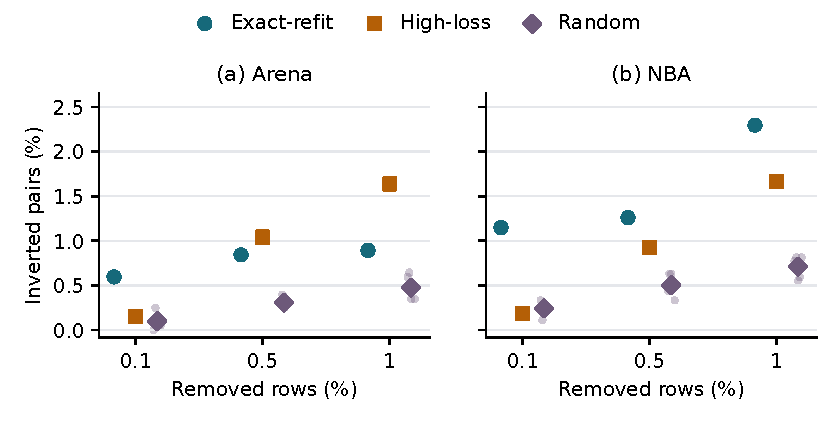
\includegraphics[width=\textwidth]{figures/dataset_budget_comparison.pdf}
 \caption{Budget-resolved disruption on (a) Arena and (b) NBA, with a shared vertical scale. Solid markers show deterministic values or random-mask means; faint random markers show the five seeds, not uncertainty bounds. Removed-row counts are Arena: 38/190/381; NBA: 41/207/414. Input-order controls are not plotted as additional replicates.}
 \label{fig:budgets}
 % @evidence[[paper_data.json#/final_evaluation/evaluation_evidence/episodes]]
\end{figure}

The measured contrast is consistent with a restricted interpretation of the selector. Its ranking of contenders prioritizes the clean leader, while high-loss deletion can perturb other parts of the order. That mismatch makes uniform superiority on all-pairs inversions unnecessary. It does not, however, explain the observed dataset difference causally: the exports do not contain a controlled decomposition of which criterion, contender, or graph property accounts for the difference. Nor does the response to these budgets identify the smallest deletion sufficient for any specific reversal.

\subsection{Fixed-mask resampling preserves a cross-setting contrast}
Figure~\ref{fig:conditional} displays every unique stored conditional gain. All high-loss-relative gains are negative on Arena and positive on NBA. In percentage-point units, the Arena gains range from $-0.794$ to $-0.231$, with mean $-0.504$; the NBA gains range from $0.222$ to $1.950$, with mean $0.806$. The aggregate advantage therefore cannot be promoted to an unconditional statement that this selector is a stronger deletion rule on both datasets. Under the documented reweighting, the relative disruption remains setting-dependent.
% @evidence[[paper_data.json#/final_evaluation/evaluation_evidence/episodes/0/solution/conditional_group_bootstrap]]

Relative to fixed random masks, Arena gains include negative values, ranging from $-0.215$ to $0.496$ percentage points. NBA random-relative gains are positive throughout the stored records, ranging from $0.592$ to $2.295$ percentage points. These ranges describe the recorded draws, not confidence limits or a probability of future superiority. All stored draws completed their weighted refits; duplicated exports add no additional evidence about that variability.
% @evidence[[paper_data.json#/final_evaluation/evaluation_evidence/episodes/0/solution/conditional_group_bootstrap]]

\begin{figure}[t]
 \centering
 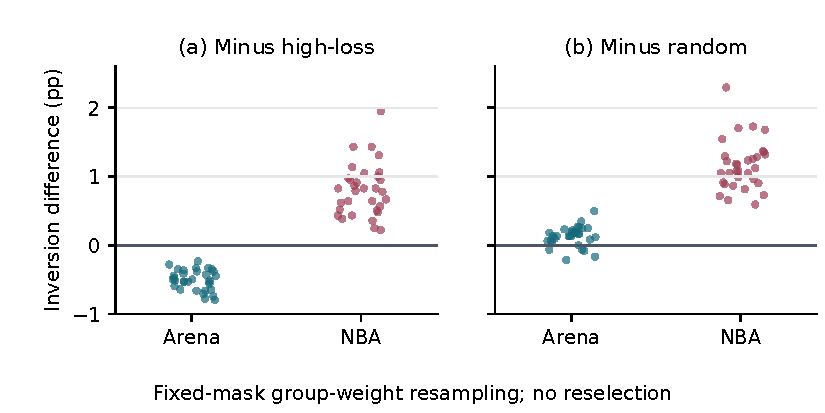
\includegraphics[width=\textwidth]{figures/conditional_resampling_contrasts.pdf}
 \caption{Conditional differences in mean inversion disruption, exact-refit minus (a) high-loss or (b) random deletion. Each dataset contributes its 32 unique group-weight draws; horizontal jitter only separates points. Dataset colors have the same meaning in both panels. The zero line denotes equal disruption. Masks remain fixed, weighted removed mass varies, and no selection is repeated. These are not full-procedure confidence intervals.}
 \label{fig:conditional}
 % @evidence[[paper_data.json#/final_evaluation/evaluation_evidence/episodes/0/solution/conditional_group_bootstrap]]
\end{figure}

The seed-resampling endpoints address a narrower source of randomness. For the aggregate gain over random deletion, they are $[0.007378,0.008169]$ in inversion-fraction units. For the high-loss-relative gain, both endpoints equal 0.002382 because the compared curves are deterministic across seeds. This equality is not evidence of negligible data uncertainty: the conditional reweighting results visibly change the gains and expose opposite dataset orderings. Conversely, the conditional draws do not supply uncertainty for a deletion rule that could adapt its masks after reweighting.
% @evidence[[paper_data.json#/final_evaluation/metrics/paired_gain_random_ci_low]]
% @evidence[[paper_data.json#/final_evaluation/metrics/paired_gain_random_ci_high]]
% @evidence[[paper_data.json#/final_evaluation/metrics/paired_gain_disagreement_ci_low]]
% @evidence[[paper_data.json#/final_evaluation/metrics/paired_gain_disagreement_ci_high]]

\subsection{Numerical checks and configuration evidence}
The no-deletion curves have zero disruption, and reversing input order leaves every recorded method curve unchanged within its seed and dataset. These checks support a numerical and indexing interpretation of the reported comparisons rather than an artifact of row order or refitting unchanged data. They do not establish completeness of the deletion search, realism of an adversary, or adequacy of the statistical model. The source-defined certificate checks were satisfied in the completed final evaluation; candidate-generated auxiliary descriptions remain unverified.
% @evidence[[paper_data.json#/final_evaluation/evaluation_evidence/episodes]]
% @evidence[[paper_data.json#/grounding_sources/final.qualification.outcome]]

Development configurations are informative only as descriptive context. They share influence-prefix constraints but differ in how contenders are screened or refitted. A tied development aggregate for the bounded exact-refit and retained-curvature configurations does not show identical masks, equal runtime, or equivalence on the final partition. No final controlled ablation estimates the effect of replacing the shortlist rule while holding the rest of the evaluated procedure fixed. We therefore attribute the final measurements to the evaluated configuration as a whole.

\section{Discussion and Limitations}
\paragraph{What the audit establishes.}
A deletion witness demonstrates that a particular fitted ranking is dependent on a particular subset of observed outcomes under a stated objective. Independent refitting makes that finite perturbation observable. Normalization by the number of participant pairs helps compare lists of different lengths, but assigns equal weight to all pair inversions, including changes far from the top. A ranking with a small global inversion fraction can still change an important local comparison. The secondary leader metric partly addresses this issue, without supplying a complete account of top-rank uncertainty.

\paragraph{What the comparison does not isolate.}
Arena and NBA differ in participants, comparison density, outcomes, content dependence, time span, and preprocessing. Their different responses cannot be attributed to crowd voting versus sports competition alone. The historical team-code model is static across eras, and the largest-component filter changes which participants are included. Equal row fractions do not remove these confounds. No matched-support intervention, expert-versus-model-judge study, or graph-property ablation is available. The scientific conclusion is conditional on these retained graphs, budgets, objective, and deletion rules.

\paragraph{Restrictions of selection and uncertainty.}
The contender shortlist is bounded; within-contender orders remain fixed; selection favors leader demotion rather than the reported all-pairs objective. A weak result can arise from any of these restrictions, and the present evidence does not separate them. The group-weight diagnostic respects declared content groups, not all possible crossed dependence. It holds masks fixed and uses a single stored random-mask family. It neither adjusts for development selection nor supplies uncertainty for attack reselection. No ridge-sensitivity experiment, full adaptive uncertainty procedure, or runtime comparison is reported.

\paragraph{Sensitivity is not a confidence statement.}
The deletion comparison and the uncertainty diagnostic have different reference objects. A deletion witness compares a retained fit with the original clean fit. A weighted draw instead compares weighted retained fits with a newly fitted weighted clean ranking. Thus a change in a conditional gain need not mean that the same participant pair crossed the same original boundary. Rank inversion is also discontinuous in fitted scores: a small score displacement near a tie can change the order, whereas a larger displacement away from a tie may not. The measured inversion fraction cannot by itself identify either the score margin or practical importance of the affected comparisons. Reporting the full budget-resolved curves together with their conditioning assumptions is more informative than treating an aggregate gain or a seed interval as a universal stability certificate.

\paragraph{Reproducibility and responsible interpretation.}
The supplied source snapshots, normalized resources, evidence exports, and figure-generation script support inspection and regeneration of the reported summaries. A complete raw-source-to-partition builder and the original raw archives are not included in the staged materials, so end-to-end reproduction from raw public data remains incomplete. Supplementary Information distinguishes this gap from reproducible figure extraction. The analysis is retrospective: it does not demonstrate access to live votes or practical manipulation of any deployed leaderboard. Results should motivate transparent reporting of sensitivity, not claims that a model's quality or a team's ability changed when observations were removed.

\section{Conclusion}
This study evaluates fitted-ranking sensitivity through constrained row deletion and independent refitting. Clean influence orders define checkable nested subsets, while bounded retained-data selection chooses among contender-specific prefixes. On the recorded final partitions, the evaluated configuration yields greater aggregate pairwise disruption than high-loss and random deletion. The more informative result is the lack of uniformity: high-loss deletion is more disruptive at the larger Arena budgets, whereas the studied selector exceeds it throughout the measured NBA budgets. Conditional group-weight resampling retains opposite high-loss-relative signs across these settings.

These findings support reporting sensitivity as a dataset-, budget-, and intervention-specific property. They do not identify a globally minimal perturbation, validate an unrestricted attack, or isolate a causal effect of evaluation design. A useful extension would preserve independent refitting while comparing matched supports, alternative ranking objectives, and a fully repeated selection procedure under dependence-aware resampling. Those extensions are not measured here. For current use, the warranted conclusion is narrower: an aggregate disruption advantage can coexist with meaningful comparator reversals and conditional uncertainty that should remain visible to readers.
% @evidence[[paper_data.json#/final_evaluation/evaluation_evidence/episodes]]

\clearpage
\bibliography{references}
\bibliographystyle{paper}

\clearpage
\appendix
\section{Supplementary Information}
\subsection{Retained-mean objective and numerical implementation}
The readable selector source preserves ordered endpoint counts and fractional wins, which are sufficient statistics for the objective actually fitted. Both the gradient and Hessian are normalized by the retained row count. Newton updates are centered; a Cholesky solve supplies the direction; backtracking accepts sufficient decrease or a roundoff-tolerant decrease accompanied by a smaller gradient. Fitting starts at zero for the clean dataset and uses a previous retained fit as a warm start for larger nested deletions. The removed-set cache avoids repeating a fit when prefixes coincide.

The selector allows up to 100 Newton iterations, seeks maximum absolute gradient below $10^{-11}$, and rejects a returned fit above $10^{-9}$. Backtracking permits 30 step reductions. The independent L-BFGS-B configuration allows 1,000 iterations, with gradient tolerance $10^{-10}$, function tolerance $10^{-15}$, and 40 line-search steps. Its accepted gradient residual is at most $2\times10^{-7}$. These are source-defined numerical settings, not measurements of solver efficiency.
% @evidence[[source_evidence/selector.py#L84]]
% @evidence[[source_evidence/evaluate_final.py#L667]]

Ranks use scores rounded to eight decimal places and participant identity for ties. Influence orders use values rounded to ten decimal places and stable row keys for ties. The clean certificate requires mean score below $10^{-7}$ in absolute value, a gradient residual below $2\times10^{-7}$, and maximum score difference from the independent fit below $2\times10^{-4}$. The Hessian-solve residual must be below $2\times10^{-7}$ and influence differences below $2\times10^{-6}$. Prefix membership is checked exactly against recomputed stable-key orders at the declared budgets.
% @evidence[[source_evidence/evaluate_final.py#L680]]
% @evidence[[source_evidence/evaluate_final.py#L706]]

For a contender $c$, define clean gap $h_c=\widehat\theta_l-\widehat\theta_c$ and retained gap $h_{cf}$. The tuple used for both screening and retained-data selection is
\begin{equation}
 \left(\sum_f\operatorname{rank}_{cf}(l),\quad
       \sum_f\mathbf{1}\{h_{cf}<-10^{-8}\},\quad
       \sum_f\operatorname{clip}\left[\frac{h_c-h_{cf}}{\max(h_c,10^{-8})},0,2\right],\quad
       -\operatorname{rank}_{D}(c)\right).
\end{equation}
% @evidence[[source_evidence/selector.py#L145]]
Ranks in this tuple are zero-based. Screening substitutes predicted retained scores. The shortlist helper retains the screening maximizer and runner-up and fills available slots by screening score. Final selection is lexicographic over complete retained fits. Nothing in the exported evidence identifies which internal tie-break determined an observed result, so no such attribution is made.

\subsection{Data partitioning and source provenance}
The Arena snapshot is \path{lmarena-ai/arena-human-preference-55k} at commit \nolinkurl{18c298340948c0e7f7727399fd459cca6ce0ca6f}; its supplied raw CSV SHA-256 is \nolinkurl{0692154aaf20fc6649090c3f49b6b5dd1e693a765ecb5f0856ae0da5946f5be2}. The NBA source is \path{fivethirtyeight/data}, commit \nolinkurl{4c1ff5e3aef1816ae04af63218015066e186c147}, file \path{nba-elo/nbaallelo.csv}, with SHA-256 \nolinkurl{d46ed3540ee8d9eca31b3e94cc8c777e0be5156173d814ebf65b8195e8d616bc}. Source licenses are Apache-2.0 and CC-BY-4.0, respectively. These identifiers are provenance, not evidence that every processing detail can be reconstructed from the public files alone.
% @evidence[[source_evidence/manifests/arena_manifest.json]]
% @evidence[[source_evidence/manifests/nba_manifest.json]]

The recorded normalization applies NFKC and Unicode whitespace collapse to parsed text turns; missing values become empty strings and empty turns are conservatively grouped. Arena grouping connects rows sharing any normalized prompt or response turn or normalized raw example, before outcome extraction. NBA uses normalized date, sorted original team codes, and aligned scores, retaining only \texttt{\_iscopy=0}. Partition membership hashes the fixed split identifier, dataset family, and group; hash residue below 30 modulo 100 is assigned to development, with the complement final. Largest connected components are selected within each partition.
% @evidence[[source_evidence/manifests/arena_manifest.json]]
% @evidence[[source_evidence/evaluate_final.py#L769]]

The final manifests record 38,192 retained Arena rows and 41,418 retained NBA rows. NBA excludes 2,898 rows outside its retained component; Arena excludes none at this component-filtering step. Both manifests report zero cross-partition content and source-identity intersections. These checks concern the declared normalization and source identifiers, not unobserved dependence. Historical NBA identities are team codes rather than a harmonized franchise-by-era model. A manuscript-side source inventory and regeneration commands appear in \path{REPRODUCIBILITY.md}.
% @evidence[[source_evidence/manifests/arena_manifest.json]]
% @evidence[[source_evidence/manifests/nba_manifest.json]]

\subsection{Numerical and input-order controls}
Recorded no-deletion inversion curves are identically zero. Each seed contains Arena and NBA cases in canonical and reversed input order; corresponding method curves agree. The evaluator additionally checks rejection of a constant invalid certificate when the zero-score gradient is nonzero, verifies valid clean certificates, and enforces independent refits. Stored control records pass. The authoritative final record states that evaluation completed and its qualification outcome passed. This is a statement about the tested execution and acceptance checks, not a proof of unrestricted statistical validity, generalization, or causal mechanism.
% @evidence[[paper_data.json#/final_evaluation/evaluation_evidence/episodes]]
% @evidence[[paper_data.json#/grounding_sources/final.qualification.status]]
% @evidence[[paper_data.json#/grounding_sources/final.qualification.outcome]]

\subsection{Descriptive development configurations}
\begin{table}[h]
 \centering
 \begin{tabular}{lr}
 \toprule
 Configuration & Development disruption \\
 \midrule
 Clean-Hessian selection & 0.0132403 \\
 Bounded exact-refit selection & 0.0159553 \\
 Retained-curvature expansion & 0.0159553 \\
 \bottomrule
 \end{tabular}
 \caption{Descriptive development aggregates, separate from the final-partition results. These are not replicated final controlled ablations, and the tied aggregate does not imply equivalent behavior or equal computation.}
 \label{tab:development}
 % @evidence[[paper_data.json#/grounding_sources/result.top_program_03]]
 % @evidence[[paper_data.json#/grounding_sources/result.top_program_01]]
 % @evidence[[paper_data.json#/grounding_sources/result.top_program_02]]
\end{table}
Readable snapshots \path{source_evidence/clean_hessian_selector.py} and \path{source_evidence/expanded_selector.py} document the comparison configurations. The former selects using clean-Hessian predictions without the bounded retained-data finalist comparison. The latter uses a retained-curvature proxy pool of at most 24 contenders and at most 12 exact finalists, preserving the bounded selector's finalists. This source evidence establishes the configured differences, not the reason for the recorded scores. Selection from development evidence can induce optimism; the final partition is reported separately, and no development-selection-adjusted interval is available.
% @evidence[[source_evidence/clean_hessian_selector.py]]
% @evidence[[source_evidence/expanded_selector.py]]

\subsection{Conditional uncertainty and complete stored contrasts}
The uncertainty routine uses random seed 709237. It draws 256 resamples of the five seed-level means to compute the 2.5th and 97.5th percentiles reported in the main text. Separately, for each dataset it draws 32 multinomial provenance-group weight vectors and refits the clean and deleted weighted datasets. It uses the first unpermuted stored mask family, rather than pooling masks from all seeds. The same group-weight block is duplicated in each seed export; the table below contains only the unique block. Zero-weight observations remain represented through their weight, and weights on selected mask rows are set to zero before retained fitting. Normalization uses total retained weight.
% @evidence[[source_evidence/evaluate_final.py#L831]]
% @evidence[[paper_data.json#/final_evaluation/evaluation_evidence/episodes/0/solution/conditional_group_bootstrap]]

\begin{table}[h]
 \centering
 \small
 % @evidence[[paper_data.json#/final_evaluation/evaluation_evidence/episodes/0/solution/conditional_group_bootstrap]]
 \begin{tabular}{rrrrr}
 \toprule
  & \multicolumn{2}{c}{Arena} & \multicolumn{2}{c}{NBA} \\
 Draw & vs. high-loss & vs. random & vs. high-loss & vs. random \\
 \midrule
 1 & -0.794 & +0.066 & +0.827 & +1.222 \\
 2 & -0.661 & +0.265 & +0.666 & +1.123 \\
 3 & -0.496 & +0.182 & +0.518 & +1.074 \\
 4 & -0.331 & +0.066 & +1.049 & +1.283 \\
 5 & -0.562 & +0.116 & +1.432 & +1.678 \\
 6 & -0.529 & +0.000 & +1.432 & +1.728 \\
 7 & -0.496 & +0.496 & +0.568 & +0.889 \\
 8 & -0.380 & +0.347 & +0.432 & +0.901 \\
 9 & -0.364 & +0.165 & +1.135 & +1.703 \\
 10 & -0.231 & +0.132 & +0.642 & +0.963 \\
 11 & -0.711 & -0.215 & +1.308 & +1.543 \\
 12 & -0.513 & +0.182 & +0.247 & +0.654 \\
 13 & -0.413 & +0.182 & +1.061 & +1.049 \\
 14 & -0.529 & +0.033 & +0.827 & +1.234 \\
 15 & -0.661 & +0.265 & +0.222 & +0.716 \\
 16 & -0.446 & +0.198 & +0.383 & +0.592 \\
 17 & -0.380 & +0.132 & +0.950 & +1.358 \\
 18 & -0.281 & +0.083 & +0.864 & +1.172 \\
 19 & -0.777 & +0.198 & +0.913 & +1.074 \\
 20 & -0.479 & -0.066 & +0.481 & +0.815 \\
 21 & -0.645 & +0.099 & +0.358 & +1.049 \\
 22 & -0.331 & -0.083 & +0.827 & +1.185 \\
 23 & -0.430 & -0.165 & +0.975 & +1.259 \\
 24 & -0.513 & +0.165 & +0.777 & +1.296 \\
 25 & -0.744 & +0.132 & +0.617 & +0.864 \\
 26 & -0.529 & +0.248 & +0.642 & +0.728 \\
 27 & -0.529 & -0.066 & +0.950 & +1.320 \\
 28 & -0.347 & +0.248 & +0.790 & +0.913 \\
 29 & -0.347 & +0.132 & +1.000 & +1.370 \\
 30 & -0.595 & +0.231 & +0.506 & +1.049 \\
 31 & -0.645 & +0.215 & +0.432 & +0.987 \\
 32 & -0.446 & +0.132 & +1.950 & +2.295 \\
 \bottomrule
 \end{tabular}
 \caption{All unique stored conditional gain records in percentage points. Positive values mean greater disruption for the studied selector. Draw indices are identifiers, not additional experimental conditions. These fixed-mask weighted refits do not estimate uncertainty for reselection.}
 \label{tab:bootstrap}
\end{table}

\subsection{LLM Usage}
LLM assistance was used for research-question development, generation and revision of candidate analysis code, reference-query planning, source inspection, manuscript drafting, and manuscript-side plotting and validation code. Numerical comparisons reported here originate from the supplied evaluation artifacts, not from LLM predictions or invented measurements. The paper-writing process did not rerun the scientific evaluation or add new experimental conditions. Reference records and available abstracts were consulted using exact identities; citation traversal and broad leaderboard-deletion searches were not used. Model identities and human oversight not established by the supplied process record are not inferred. The incomplete raw-data reconstruction path remains a limitation despite automated assistance.

\end{document}
